% Template DFG-Sachbeihilfe-Antrag
% Version Aug 2014
% Autor: Fabian schneider, VISUS 
% erstellt auf Basis einer Vorlage von Markus Huber, Corinna Vehlow und Marco Ament
% ursprüngliches Template: Stephan Wenger

\documentclass{dfg_en}
\usepackage[utf8]{inputenc}
\usepackage[english]{babel}
\usepackage{eurosym}
\usepackage{amsmath,amssymb,amsfonts,amsthm} % mathematische Symbole
\usepackage{graphicx}  % notwendig für die Einbettung von Grafiken.-graphics ist ein ganzes Bündel und enthält auch graphicx
\usepackage{color}
\usepackage{setspace}
\usepackage{lmodern}  % Alternative zur palatino Schrift
\usepackage{textcomp,gensymb} % umfangreiche Pakete fuer Symbole wie \micro, \ohm, \degree, \celsius etc.
%\usepackage{subfig}  % Um Abbildugnen mit Subfigures erstellen zu können
\usepackage{subfigure}
\usepackage{calc}   % ermoeglicht Rechnen mit Laengen und Zaehlern
\usepackage[plain]{fancyref}
\usepackage{helvet}
\usepackage{microtype}
\usepackage{pdfpages}
\usepackage{currvita}
%\usepackage[babel,german=guillemets]{csquotes}
\usepackage{titlesec} % provides titlespacing
\usepackage{multicol}
\usepackage{xcolor}
\usepackage{tabularx}

% Labels for objectives - BEGIN
\newcounter{objectives}
\makeatletter
\newcommand\objective[1][]{\item[#1]\refstepcounter{objectives}\def\@currentlabel{#1}}
\makeatother
% Labels for objectives - END

% Labels for RQs - BEGIN
\makeatletter
\newcommand\rqs[1][]{\item[#1]\def\@currentlabel{#1}}
\makeatother
% Labels for RQs - END

\usepackage{enumitem}

% Disable single lines at the start of a paragraph (Schusterjungen)
\clubpenalty = 10000
% Disable single lines at the end of a paragraph (Hurenkinder)
\widowpenalty = 10000 \displaywidowpenalty = 10000

% References
\usepackage[style=numeric-comp,bibstyle=numeric,sorting=none,date=short,backend=bibtex,isbn=false,url=false,doi=false,eprint=false,defernumbers=true,maxnames=9,minnames=5,firstinits=true]{biblatex}
\addbibresource{references.bib}
\DeclareBibliographyCategory{publikationen}
\DeclareBibliographyCategory{publikationen-andere}
\DeclareBibliographyCategory{patente-angemeldet}
\DeclareBibliographyCategory{patente-akzeptiert}
\newcommand*{\addtopub}[1]{\addtocategory{publikationen}{#1}\nocite{#1}}
\newcommand*{\addtopubandere}[1]{\addtocategory{publikationen-andere}{#1}\nocite{#1}}
\newcommand*{\addtopatangemeldet}[1]{\addtocategory{patente-angemeldet}{#1}\nocite{#1}}
\newcommand*{\addtopatakzeptiert}[1]{\addtocategory{patente-akzeptiert}{#1}\nocite{#1}}
\DeclareBibliographyCategory{publikationen_juerjens}
\newcommand*{\addtopubju}[1]{\addtocategory{publikationen_juerjens}{#1}\nocite{#1}}
\DeclareBibliographyCategory{publikationen_schneider}
\newcommand*{\addtopubschn}[1]{\addtocategory{publikationen_schneider}{#1}\nocite{#1}}
\renewcommand{\bibfont}{\normalfont\scriptsize}

\graphicspath{figures}

% Links and references
\definecolor{bluecol}{rgb}{0.03,0.05,0.15}
\usepackage[colorlinks, urlcolor=bluecol, citecolor=black, linkcolor=bluecol, pdfborder={0 0 0}, pdfpagemode=UseNone]{hyperref}
% For autoref
\addto\extrasenglish{  
	\def\sectionautorefname{Section}  
}

%\newcounter{wp}
%\newcounter{subwp}[wp]
%\renewcommand\thesubwp{\thewp.\arabic{subwp}} 
%\newcommand{\newwp}{\refstepcounter{wp}}
%\newcommand{\phase}[1]{\refstepcounter{wp}\subparagraph{PHASE~\thewp: #1}}
%\newcommand{\wpackage}[1]{\refstepcounter{subwp}\subparagraph{WP~\thesubwp: #1}}

%\newcommand{\wp}[2]{\paragraph*{{\color{#2}\rule[-1pt]{10pt}{10pt}} #1}\vspace{-0.3cm}}
\newcommand{\mywp}[2]{\subparagraph{{\color{#2}\rule[-1pt]{5pt}{10pt}} #1}}
\definecolor{color_wa1}{HTML}{5B9BD5}
\definecolor{color_wa2}{HTML}{70AD47}
\definecolor{color_wa3}{HTML}{009999}

\newcommand{\emptysection}{}
\newcommand{\emptyheading}{ \mdseries--- Not applicable.}

\newenvironment{costs}[1][]{
\newcommand{\totals}[1]{\cline{3-3} & & \textbf{##1}}
\begin{center}
\begin{tabular}{lrr}
{\bfseries #1} & pro Jahr~~ & gesamt~~ \\
\hline
}{
\end{tabular}
\end{center}
}

\newenvironment{costshardware}[1][]{
\newcommand{\totals}[1]{\cline{2-2} & \textbf{##1}}
\begin{center}
\begin{tabular}{lr}
{\bfseries #1} & gesamt~~ \\
\hline
}{
\end{tabular}
\end{center}
}

\definecolor{redcol}{rgb}{.7,0,0}
\definecolor{bluecol}{rgb}{0,0,.8}
\newcommand{\remark}[1]{\emph{{\color{bluecol}\textbf{REMARK:} #1}}}
\newcommand{\myldots}{\colorbox{black!20}{{\color{black!60}[...]}}}
\newcommand{\citreq}{\colorbox{yellow!60}{{\color{redcol}[\emph{citation?}]}}}
\newcommand{\email}[1]{\href{mailto:#1}{#1}}

\usepackage{todonotes}
%\usepackage[disable]{todonotes}

\newcommand{\motivation}[1]{{\scriptsize\textbf{[Motivation:]}} #1}
\newcommand{\method}[1]{{\scriptsize\textbf{[Method:]}} #1}
\newcommand{\results}[1]{{\scriptsize\textbf{[Result:]}} #1}

\begin{document} % max. 20 Seiten

%\listoftodos

% -----------------------------------------------------------------------------------

\formattitle{Prof. Dr. Jan Juerjens, Universität Koblenz-Landau, Koblenz, Germany \\ 
	Prof. Dr. Kurt Schneider, Leibniz Universität Hannover, Hannover, Germany
	\\
\\
TraceSEC -- Tracing Security in Software Engineering}

% -----------------------------------------------------------------------------------

\begin{figure*}[b!]
	
\includegraphics[width=\columnwidth]{dfg_address}
\end{figure*}
\vspace{1em}
%!TEX root = Beschreibung_des_Vorhabens.tex

\subparagraph*{Motivation and Context:}
Software is often unnecessarily insecure. While developers tend to be sensitive to security issues in highly sensitive domains, developers in ordinary software projects are often unfamiliar with security aspects. For example, the correct implementation of security-critical functionalities REFfiresmith2003 REFtondel2008 is not always ensured. There are only a few security experts available who cannot assist in all projects. Guidance for developers is limited and often not tailored to a specific context. Security must be considered from the beginning of the development and throughout all subsequent phases and activities. Both, individual developer and the organization at large should increase their security competency for facing new attacks and challenges. Currently, security-specific techniques focus on security alone. They are poorly integrated with ordinary development tools and practices. Furthermore, security relevant information is scattered all around the system. Learning is treated separately and, thus, is often neglected. There is little time and inclination for external training, as the transfer from training examples to the real application context is a hurdle. Since development, problem solving, and continuous learning are not integrated, they do not benefit from each other.  

\subparagraph*{Research Vision:}
In an ideal case, existing tools or artifacts like quality models can be used to capture and refine security-related requirements and to follow the development process through all stages of develop­men. In parallel, a software development organization and their tools need to learn from their previous security problems and solutions as well as changes in public knowledge. We envision an innovative approach for integrating three core activities:

\begin{enumerate}
    \item the development of software which is potentially security relevant, 
    \item diagnosis and analysis of problems and attacks within a cycle of continuous improvement, and 
    \item use, reuse, and exploitation of security knowledge and insight in a socio-technical way.
\end{enumerate}

All levels and phases of software development must be covered, including informal early requirements and prioritization, as well as formalization and heuristic checking of security properties with respect to the initial informal demands. 

We want to investigate the potential of extending quality models and combining them with an exten­ded and adapted tracing technique. Quality models and specific artifacts are tied together by tracing development activities at a very fine-grained level. Those same tools (extended quality model and tracing) will be reused for all three core activities. Individual and organizational learning will benefit from concrete and contextualized examples that are generated as by-product of the two other tasks. These types of learning are different from machine learning.

\subparagraph*{Key Contributions:}
We extend both quality models and tracing in order to cover informal and formal activities in a socio-technical environment. This scope includes developers, customers, but also code and monitoring. Development, problem analysis, and learning must be adjusted to support each other.

The term quality model is used for generic collections and relationships of quality aspects, such as reliability, usability, etc. in ISO 25 010. In a project, a quality model must be refined to provide concrete and measurable specifications of relevant quality attributes, such as security. We trace the refinement of informal and generic terms into more specific interpretations (e.g. from performance to run-time performance of a module). This will require manual entries and automated monitoring. Extended quality models will cover the entire spectrum, but only selected relevant aspects should be included, which is difficult to decide. Tracing will span over human interaction and decision-making on informal levels down to technical monitors and metrics. Extended tracing covers a socio-technical development environment. We will optimize strategies for collecting traces for low effort and develop heuristics to identify relevant parts. Relevance also refers to the three above-mentioned activities of development, problem analysis, and learning from concrete examples.

Traceability benefits from a predefined development process, as it can be used to interpret activities and traces. We plan to integrate our approach into standard/waterfall-based and agile processes and investigate how and to which degree the intended methodology can serve those types of process.

\subparagraph*{Challenges to be Overcome:}
It will be challenging to identify what is relevant in the informal, formal, heuristic, and measurable facets of security in a specific application since there are people and artifacts involved, and they are connected via traces. The contribution of reducing manual labor to the indispensable minimum creates a tension with the effectiveness of the tracing approach. The overarching opportunity and challenge will be to reuse results from one of the above-mentioned activities to the others. This is a key concept in this proposal.
Planned Validation: A first step in evaluating the feasibility of the TraceSEC approach will show whether results from one activity can be adapted and reused to facilitate the other activities. We will provide a set of examples and use cases to demonstrate how manual and automated steps are interrelated. We will point out and investigate how an extended quality model and extended traces can be built as a by-product of software development activities, and how educational material can be derived from it. We will complement feasibility demonstrations by within-subject studies in which we empirically study how traditional develop­ment activities perform compared to those supported by TraceSEC. After the experimental comparison, we will interview subjects for their preference and perceived differences. We will triangulate perceived problems with objective indicators collected in the experiment. Long-term effects are difficult to study; we will use a case study to observe what happens to quality model and traces over several months.

\subparagraph*{Research Impact and Measure of Success:} The case below is a showcase for explaining our concepts and will later be used for demonstrating the feasibility of our approach. This case provides a context to instantiate all aspects of formal and informal, as well as all relevant activities (development, problem analysis, learning). In particular, it helps us to illustrate the techniques for reusing results across these activities: How can a similarity measure between problem cases help to find an older case as an inspiration to solve a new problem? How can we identify recommended next steps to a novice developer, based on earlier successful cases? How can educational material (e.g. screen videos) be generated from traces and connected artifacts? These questions will advance research. We intend to publish in both software engineering and security venues (conferences and journals). Specific human-centered software engineering communities will show the interdisciplinary impact of our work.

\paragraph*{A Realistic Case as Running Example}
In many projects, security issues can have dramatic consequences. For example, in December 2019 a bug in a router led to 20,000 patient records to be publicly available~\cite{ct2019a}. One of the main security issues was insufficient access control for the patient data. There was no internal access control implemented, and everyone who was in the network of the doctor’s office had access to all patient data. Due to the bug in the router, there were open ports which allowed everyone beyond the office to get into the network from the outside and to access the patient data. 

For discussion purposes, we assume a fictive software company that is going to implement a secure management system for patient data in this example. 

At first, they are collecting requirements the system has to meet. Besides considering classical functional and non-functional requirements, domain specific requirements from relevant standards must be observed, such as IEC 62304 and IEC 62366 for medical device software. Customer requirements must be checked for security implications, e.g. by automatically recommending and including relevant standards. As the project is dealing with personal data, implementing an appropriate access control is an example of such a security-implied requirement.

In system design, the architecture has to address all requirements captured. As a consequence, the required access control has to be reflected in the systems architecture. In the above-mentioned real system, access control for preventing outside attackers had been considered (including a router with firewall), but no access control for inside attackers had been planned. Such missing or neglected security mechanisms, as well as flawed and insecure security mechanisms, should be automatically detected at design time. This is a case of heuristic identification of conceptual or design problems during development. It requires a representation, that is formal enough for automated search.

The next pitfall for our fictive company occurs during implementation. The company skips the implementation of a (previously required) security mechanism to save time and effort. In addition, an unexperienced developer again selects an outdated and unsecure mechanism, e.g., a deprecated cryptographic hash function. Automated support for developers monitoring source code for security issues could warn, providing relevant documentation and best practices but also in generating at least stubs for the required security mechanisms. With respect to our TraceSEC concepts, it would be important to follow and trace security-related requirements through all steps and artifacts for identifying glitches like this. If a security-related design concept like access control has no trace to an adequate part of the implementation, a heuristic warning can be issues.

Configuration of the system is yet another important part. In addition to internal access control, the company also implemented a limitation of accesses per hour to harden the system against brute force attacks. However, the pre-configured number of accesses per hour might lead to a denial of service if the software is used without adaption to the context – e.g. a big hospital instead of a small doctor’s office.

At run-time, changes in the security assumptions will occur. For example, it has been recently shown that SHA1 has become an insecure hash algorithm due to new attack knowledge. New requirements may also be stimulated by unexpected observations at run-time, like several hundred access attempts from a single IP-address which leads to all accesses being blocked by the above-mentioned access limit. Requiring dynamic IP-address filters could be a decision by the human experts. This account of technical problems and solution attempts should be retrieved in a future case with similar profile for informing problem analysis. We also foresee the opportunity to use a sequence of decisions, consequences and artifacts, as a real-case contextualized example for developers who try to learn more about security within the scope of their particular tasks and company.

\paragraph*{Different perspectives and experience in collaborating}
The applicants and their research groups approach the topic from different angles: Jan Jürjens and his team has a long record of security modeling (e.g., in UMLsec [12]) and formal techniques to verify REF and ensure security REF. Kurt Schneider and his group focus on socio-technical aspects of software engineering, such as elicitation and validation of requirements, knowledge management [26] or explainability [5]. They build tools to support the collaboration of technology and humans in a software engineering context (e.g., FOCUS [21] [24], AppForMeetings, HeRA [27]). The collaboration of both groups started in 2008, and has been intensified over the years: From publications on detecting security-related requirements [11] to SecVolution in the DFG Priority Programm 1593  [8] [35] [33]. The successful cooperation demonstrated and strengthened the ability to join their very different competencies in the area of security within software engineering. This encourages the applicants to now go far beyond the previous common work and address a topic at the intersection of informal and formal, as well as technical and socio-technical issues. The key concept of combing that with individual and organizational learning benefits from the rare case where diverse skills and viewpoints have reached maturity in collaboration [9]. This encourages us to jointly address the challenges of TraceSEC and reach results none of the groups could reach by itself

\section{State of the art and preliminary work}
\label{sec:state_of_the_art}

%!TEX root = Beschreibung_des_Vorhabens.tex
In the following, we present the state of the art and preliminary work structured according to the five main research areas relevant for this proposal.

\vspace{-0.5em}
\subsubsection*{Security in Diverse Project Environments}
\vspace{-1em}
Advanced security engineering approaches were presented in REF?. Publications such as REF show how sophisticated monitoring and security techniques can be applied to find problems and solve them. When a new attack pattern has been identified, protection and mitigation solutions are published, e.g. in the case of nnn REF. These publications provide valuable information for security experts. Ordinary developers, however, rarely read this kind of publications. Equipped with a sound background in software development, they rely on their experience and guidance by a development process. Only a few developers are also skilled security experts. For example, the European standardization institute ETSI conducts a growing number of software and telecommunication projects with an insufficient number of security experts [11]. Therefore, developers must grow awareness and skills in security. In joint previous work, the applicants have developed an approach to identify security-related requirements in natural-language specifications [16]. When there is a flow of similar projects and specifications, Naïve Bayessian classifiers, SVP, or other machine learning mechanisms can be applied. Knauss et al. show that supervised learning from other projects is possible, but does not reach the precision and recall that can be achieved in a k-fold training and test set from a documentation from the same project and context [16]. In short, the closer a training set is to the examined body of text, the better performance can be expected.

During the two phases of the DFG Priority Project 1593, security findings were first identified in one project and used in following applications. There was a constant flow of similar inputs (specifications from the project). Our classifiers were optimized to identify security-related requirements. However, since the focus of the Priority Project was on long-living software, the focus shifted to different techniques: Natural-language processing provided the basis for identifying concepts of a two-layered security ontology, based on REFbashar. By identifying security-related terms in context of phrases, frames were used as patterns that can indicate security-related use cases or requirements. The entire approach is described in REFsg.

Every active project tends to degrade due to ad-hoc fixes and extensions. In particular, security can suffer when sensitive data is added to a software package, or when attackers find new ways of threatening the security of the system. Even an unchanged system can degrade in terms of security due to outdated assumptions about its environments [9] (see the example above). 

While our own previous work explored possibilities for machine learning several years ago REFrefsq, a learning loop assisted in gaining additional training data from past projects. Our work was focused on a specific aspect of development. It was not embedded in a development process, did not build on well-known concepts and tools such as quality models or traces, and did not address human individual learning as a key concept of merging secure development, problem analysis, and learning. 

There are several development processes that focus on security, such as Microsoft SDL REF. The process contains a list of adequate security techniques for each step of a waterfall process. Many code-level hints are provided. The process connects existing security activities in a meaningful way. However, they do not support the hand-over between different steps with respect to concrete, given security issues  WAS JETZT?. Microsoft SDL focusses entirely on security, ignoring any tradeoffs with other quality attributes. TraceSEC will make active use of security traces, e.g. by using them to generate tutorials for developers, referring to the concrete artifacts occurring in their project. They are put in perspective by the relationships induced by traces. Checklists and even tutorial videos will be generated to support development in a focused way. As a by-product, developers receive contextualized material for constant learning. A main challenge for many software projects is that the exact level of importance of the various security requirements is not known in advance and can shift as the process develops. Consideration of security issues must match and follow growing demand and growing awareness. Explicit feedback to using artifacts and techniques is an essential contribution to making security both traceable and understandable in an ordinary project. Security concerns must be embedded and integrated, however, and the effort devoted to security must be justified with respect to priorities and concrete constraints (e.g. vulnerabilities, business cases, assets). Traceability benefits from a predefined process and weaves security into it: From requirements over priorities to managing techniques, heuristics, and monitoring data.  We plan to use standard/waterfall and agile procedures as representatives of that scope and investigate how and to which degree the intended methodology can serve those representations.



\vspace{-0.5em}
\subsubsection*{Quality and Knowledge Model}
\vspace{-1em}
In many software projects, quality models are developed starting from general models, such as ISO 25 010 or Boehm’s so-called Quality Tree [4] as their quality model. This type of general models provides a structured overview of well-known software quality aspects (e.g. usability, portability) and their relationships. Quality models are often used for specifying which selection of quality aspects are particularly important for a given software. In more advanced quality models [25], general terms (e.g., security, usability) are refined to what those aspects mean in the particular project. For example, security could be refined into nnnVerschiedeneSecurityUseCases. 

Schneider [25] describes a three-layer format of quality models; the top layer contains a selection of generic quality attributes. They are selected and prioritized but terms like "usability" or "security" may still be interpreted differently between customers and stakeholders at this point. By refining those generic aspects, the second layer of the quality model contains concrete interpretations and instances of selected quality aspects, such as the design considerations mentioned in the running example. On the bottom layer, each of the concrete quality aspects is further detailed. There are heuristics and metrics for measuring the extent of meeting the respective quality requirement.  

Wagner et al. [36] describe the Quamoco approach. They claim there is no seamless integration of abstract generic terms and security measurement.  They propose richer quality models for security, similar to the layers described in [25]. They report on spending over three years’ time on bridging the gap. They suggest using GQM [3] [32] to guide the refinement process and wander whether such an endeavor is feasible in practical projects. We consider it essential to reduce effort and increasing value by recording and reusing lessons learned.

In TraceSEC, we use extended Quality Models. They are not limited to security but may contain other quality aspects. For example, usability is often competing with security: High standards for passwords, for example, may raise the bar for memorizing them. It is therefore important to prioritize aspects of usability against aspects of security.

Extended quality models contain the three levels described above and may be enriched by further intermediate results on the way from informal priorities to formal monitoring and ensuring of security properties REFkoblenz. With so much information about security centralized in one artifact, extended quality models are a rich source of examples and recommendations in similar cases. In TraceSEC, quality models are developed into a repository for storing and maintaining knowledge; knowledge about everything related to security in that project [26]. There are two dimensions in the quality model: Along the dimension of security refinement and along the dimension of development progress. Traces weave both dimensions together.

While quality models can collect intermediate results, they cannot express dependencies and temporal relationships between the different parts of the quality model. Extended quality models have a dual nature. Since we strive for extracting reusable parts from the quality model, a knowledge perspective can help: It emphasizes the need to treat parts of the quality model as pieces of knowledge. They can be used and reused in various forms (development, problem analysis, learning). Treating an extended quality model as a knowledge representation highlights its value as an asset independent of a particular project. Organizational learning relies on externalizing (e.g., by provoking breakdowns, according to Schön [20] and reusing knowledge elsewhere, and for a different purpose. 

\vspace{-0.5em}
\subsubsection*{Security-related Activities and Analyses}
\vspace{-1em}
Bugs, vulnerabilities, and code smells are among the criteria for security standards of software systems. Automated security checks and metrics are used for continuously estimating and monitoring those security standards. Platforms like SonarQuble are embedded in continuous integration approaches and can be executed without user interaction. While this permits deep insights into the system and its security aspects, tools release an excessive number of warnings. Many issues raised are of limited relevance for the project and its security.

According to the OWASP Top 10 application security risks, the most dangerous threat is the injection of untrusted data. Accordingly, a lot of works analyze calls to critical APIs, like SQL queries, and check if external data is forwarded to the APIs unfiltered or check parameter ranges. One special field for this kind of analysis are misuses of crypto APIs. Many crypto APIs are very complicated and often used in a non-secure way. As such analyses usually are very locally they might produce a lot of warnings for not that dangerous calls, as no information about the structure of the system and the requirements is available.

Another OWASP Top 10 threat is the exposure of sensitive data. Instances of this threat are usually detected using secure data flow or taint analyses. Critical data is only allowed to flow from secure sources to secure sinks. There are a lot of tools providing such analyses like FlowDroid or SuSi. Unfortunately, they have to rely on manually created or learned libraries of critical sources and sinks, making the results not perfectly suitable to the system.

All of the security issues discussed above might already have been reported as concrete vulnerabilities (CVE) and general weaknesses (CWE) have been extracted from those weaknesses. Specific implementation structures might be directly connected to well-known CWEs threatening the systems security: E.g. throwing Runtime-Exceptions threatens availability. Many tools like Checkstyle, Findbugs, SonarQube, and others check for this reason for such simple patterns and report them. Especially this very simple patterns are violated very often leading to very long reports that are usually not prioritized.

Even if the own product itself does not contain any critical security issues, its security could be at stake due to used libraries having security issues. Such kinds of issues might arise from the use of old (and maybe already known as insecure) libraries. Accordingly, there is a lot of work on analyzing the dependencies of a project and checking if they are known to have unfixed security issues.

Last but not least various security metrics have been developed for estimating parts of the system that are of high importance. Relations between security-relevant and non-security-relevant elements, might allow a prediction on the suitability of making security critical mistakes. Unfortunately, this kind of metrics usually need additional information, like the critical attributes of the system, that usually is not part of the code but is a part of the quality model discussed before.

While the approaches discussed above only focus on the implementation approaches like STRIDE, UMLsec, SecDFDs, or SecBPMN can be used to plan required security mechanisms at requirements engineering or at design-time. Their aim is to support security from design-time and to provide mechanisms for identification and planning of required security mechanisms. For this purpose, UMLsec extends UML with various security properties for the specification of security requirements. The specified security requirements can be checked for conciseness and completeness according to different security policies provided by UMLsec.

\vspace{-0.5em}
\subsubsection*{Elicitation and Interpretation of Traces}
\vspace{-1em}
During the development of software systems, developers leave traces as the make changes. Gotel et al. REF++Traceability define essential terms for the area of tracing. Jarke et al. REF found requirement tracing to be an effective bridgte that aligns system evolution with changing stakeholder needs. NnnREFanAnalysis mention several directions of tracing, e.g. information-driven in which tracing provides "the abilita to link between functions, data, reguirements ... that refers to them." They emphasize the need to focus research effort on pre-traceability, i.e.: What led to a requirement? Accoring to nnnREFmodelingOf, a project manager defines the types of traces that the project team should capture and maintain. This activity is called Trace Specification. In TraceSEC, trace selection will be focused to the initially-mentioned core activities. Their use of shared development environments like issue trackers, source code repositories, or build systems can be automatically tracked. These systems usually log developer activities and their exact date and time when an issue was created, changed, or commented, when code has been committed, or when a system build has been configured or executed. This information is stored as meta data on the corresponding content or logged in a log system. It can be collected as raw traces to be analyzed in real time or post-factum. Several authors differentiate explicitly set trace links from implicitly derived relationships between artifacts (e.g. REFcleland-hGoalCentric).

Raw traces can be helpful for measuring the product \cite{ProductMeasures} or process quality \cite{ProcessMeasures}, but they can also be interpreted to understand and evaluate developer activities  in context \cite{TraceInterpretation} and to relate development artifacts to each other. The latter creates \emph{trace links} between artifacts, which allow multiple artifacts to be analyzed together. By combining the analysis of traces (activities upon artifacts) and trace links (relations between artifacts), development activities can be understood on a higher level. Unfortunately, tracing costs can grow excessively high if trace links have to be created and maintained manually by human users, and as a result, practitioners often fail to establish adequate traceability in a project, as nnnREF+ImprovingTrace report.

In our previous work, we generate traces between software development artifacts, e.g., security requirements and system design models \cite{Houmb2009}, or design models and code \cite{Peldszus2019}.

Recording large quantities of traces may pose a challenge: First, traces need to be maintained, which adds another burden to the development process \cite{TraceMaintenance}. Second, large trace sets slow down the analysis considerably. Therefore, a balance has to be found between collecting all possible traces and collecting too few traces for the analysis. nnnREF+survey propose software producers can prove to their client that the requirements have been understood. 

In TraceSEC we collect developer activities from a variety of sources. The raw traces will be filtered, semantically grouped for interpretation and interconnected to sequences of related activities for identifying security-related interconnections between artifacts, activities or the lack thereof. There is related work on Traceability Models REFriskManagement, some of which refer to the value of tracing. Autmating of creating trace links was proposed by many authors REF, and different heuristics were described. However, reducing the effort REFsieheOben is only one side of the coin. In TraceSEC we intend to also increase the benefit REF+modeling 

\vspace{-0.5em}
\subsubsection*{Innovative Reuse of Security Knowledge}
\vspace{-1em}
There will be a wide spectrum of quality aspects, sub-aspects, and respective representations in the quality model of a specific software project. Aspects start from overall priorities and refine into security requirements, heuristics, and mechanisms. This multi-level system of formal and informal, automatable and decision-related information is currently spread over many artifacts. We envision integrating the pieces in an extended quality model, capture relationships through fine-grained traces, and treat the result as a security knowledge representation. Weaving such a complex web of interrelated items must be supported automatically, and can be justified by using and reusing it for several purposes.

In earlier work, Schneider et al. studied systematic learning from experience in companies [22] [28] [10]. The concept of an experience factory by Basili [2] was applied and adapted to suit the needs of software companies, as reported in joint work with Basili [30]. There were technical findings concerning the central repository for learning from experience [30] [23]. Reflections on the use and benefit of experiential learning in software development, key lessons learned included [23]: An efficient structure for storing new experiences is essential for a large-scale sharing of experiences in an organization. However, identifying content such as valuable observations and tacit knowledge [19] is even more critical for success. Usually, experts and experienced staff are not aware of what others need. Therefore, mechanisms to support identifying that knowledge are typically socio-technical, including technical mechanisms for supporting awareness and externalization [18] [1] [15]. 

In TraceSEC, there are two analogous challenges: (1) Identification of a piece of information that could be relevant for others. The above-mentioned challenge will be addressed by trying to use quality model entries that are provided anyway, and tie them together with fine-grained traces of activities. The latter should be collected as a by-product. Explicit comments by the experts will only be requested if there is a pattern or heuristic indicating the opportunity to capture tacit knowledge. Thus, our methods and research approach are informed by the lessons learned in the above-mentioned experiential learning. However, TraceSEC addresses security in-depth, whereas SEC explored experiential learning on a far broader and more superficial level.

The concept of a by-product is important for TraceSEC. Schneider [24] proposed a scheme of recording events in which important knowledge surfaced while some other activity was carried out anyway. Originally, the demonstration of an innovative prototype was used: Whenever a prototype is demonstrated and explained, the knowledge engrained in that prototype is complemented by the requirements and knowledge of its creator and demonstrator. Schneider [24], therefore, proposed several technical and methodological steps to record that demonstrations as run-time trace and as screen-capture video with the explanations on the audio track. Almost no additional effort is necessary, and the resulting web of traces and explanations can be exploited in several ways [24]. Other researchers have used the by-product paradigm to capture annotations in pdf documents for rationale [1] [15]. Noch ein Beispiel, SecVol?

When knowledge and learning is combined with sophisticated technical tasks, e.g. in software and security engineering, both technical and human aspects should be considered together. The optimal benefit often depends on reducing participant effort to the minimum by using more powerful support. The strength of this socio-technical situation comes from applying rather inexpensive computational power to rather informal and valuable sources of human skills that can still not be substituted by machines – partly because they refer to human experience, decisions, and values. Exploiting rich knowledge repositories for supporting humans, as in REF?, is the vision we follow.

\vspace{-0.5em}
\subsubsection*{Preliminary work}
\label{sec:preliminary_work}
\vspace{-1em}


\subsection{Project-related publications}

\subsubsection{Articles published by outlets with scientific quality assurance, book publications, and works accepted for publication but not yet published.}
%!TEX root = Beschreibung_des_Vorhabens.tex

%\todo{max. 10 publications}

\defbibheading{Pub}{\label{sec:pub}}
\vspace{-0.8cm}
\hspace{-0.95cm}
\begin{tabular}{p{8.3cm}p{8.3cm}}
	\defbibheading{PubKo}{\subsubsection*{Juerjens}}
	\addtopubju{Juerjens2018xyz}
	\printbibliography[heading=PubKo,category=publikationen_Juerjens] 
	&
	\defbibheading{PubSchn}{\subsubsection*{Schneider}}
	\addtopubschn{Schneider2013abc}
	\printbibliography[heading=PubSchn,category=publikationen_Schneider]
\end{tabular}\vspace{-0.2cm}
%\defbibheading{Pub}{\label{sec:pub}}
%\addtopub{Parnas1972Criteria}
%\printbibliography[heading=Pub,category=publikationen]

\subsection*{1.1.2--1.1.3\emptyheading}

%\subsubsection{Andere Veröffentlichungen}
%\input{1-1-2-veroeffentlichungen}
%\defbibheading{PubAndere}{\label{sec:pub-andere}}
%\addtopubandere{Shneiderman1996Eyes}
%\printbibliography[heading=PubAndere,category=publikationen-andere]

%\subsubsection{Patente}

%\paragraph{Angemeldet}
%\input{1-1-3-1-angemeldet}
%\defbibheading{PatAngemeldet}{\label{sec:pat-angemeldet}}
%\addtopatangemeldet{Shneiderman1996Eyes}
%\printbibliography[heading=PatAngemeldet,category=patente-angemeldet]

%\paragraph{Akzeptiert}
%\input{1-1-3-2-akzeptiert}
%\defbibheading{PatAkzeptiert}{\label{sec:pat-akzeptiert}}
%\addtopatakzeptiert{Shneiderman1996Eyes}
%\printbibliography[heading=PatAkzeptiert,category=patente-akzeptiert]

% -----------------------------------------------------------------------------------

\section{Objectives and work programme}

\subsection{Anticipated total duration of the project}
36 months, from 1.9.2020 to 31.8.2023.

\subsection{Objectives}\label{sec:objectives}
%!TEX root = Beschreibung_des_Vorhabens.tex
\todo[inline]{Rahmen}
In the TraceSEC project, we want to develop a semi-automated socio-technical method that combines existing and new security-related elements as a source for use and reuse in three core activities:
\begin{enumerate}
	\vspace{-0.5em} \item software development, 
	\vspace{-0.5em} \item problem diagnosis and analysis, and 
	\vspace{-0.5em} \item for continuous learning of an organization and its developers.
\end{enumerate}

The method needs to be socio-technical since it has to consider and optimize human needs and abilities together with new techniques for automating essential tasks. Those tasks include tracing of activities, extraction of relevant steps, and formalization for identifying similar cases. Combining traces with connected artifacts and parts of the quality model allows to identify meaningful scenarios. Finding and delivering scenarios similar to a current task at hand assist developers in all three core activities: (1) Development, (2) problem analysis, and (3) learning. 

We want to develop techniques and demonstrators illustrating the potential of adding value to scenarios, e.g., by turning screenshots and a sequence of steps into a security training video. Since it relies on real cases from that same environment, the problem of de-contextualization and irrelevance is addressed and mitigated: Contextualization comes for free since the scenarios come from the same context anyway. Relevance is likely, due to the fact that those cases were relevant in the past.

The method will, therefore, include a number of exemplary generators and matching algorithms or classifiers. They operate on traces, with artifacts and parts of a quality model attached as they are used. The method will integrate automated and semi-automated parts into a strategy for software-developing organizations to increase their competency and efficiency in dealing with security-related issues, yielding the following benefits:

\begin{itemize}
\vspace{-0.5em} \item They will recognize security implications on all levels represented by the quality model.
\vspace{-0.5em} \item They will widen the scope of security activities to informal (human-based) and formal (code and reasoning) aspects.
\vspace{-0.5em} \item This will allow companies to see and maintain relationships and dependencies between security-related elements and activities. They will reflect and reason about complete scenarios rather than focusing on single security challenges in isolation.
\vspace{-0.5em} \item Pattern matching will identify similar threats and scenarios. Clustering scenario traces and generating compact pieces of knowledge will make them relevant for the task at hand.
\vspace{-0.5em} \item Since we consider traces and scenarios first-class objects, they will be treated as knowledge items and reused in all three core activities, transformed to the respective purpose. This helps to make acquired knowledge relevant to the tasks at hand REF.
\end{itemize}

We suggest referring to an extended quality model as reference for security-related information and activities. The method does not rely on a certain development type (such as agile, traditional, hybrid), but can be configured to a given type. We seek to investigate the basic principles that can be mapped to various environments and development styles.

\subsection{Work programme incl. proposed research methods}
% Für jede Antragstellerin und jeden Antragsteller
%!TEX root = Beschreibung_des_Vorhabens.tex

Figure nnn shows the principal components of the TraceSEC method. The pyramid symbolizes an extended quality model [26] REFanderes as described above. Since the selection, order, and details of those activities may differ between projects, TraceSEC will enable projects to map and configure respective parts of their development approach to the TraceSEC reference model. This is also used to accommodate various development styles.

Activities referring to a quality model (WP1) impose traces between quality model, other artifacts, and the activities (WP2). Raw traces gained from recording basic interactions must be reduced to a subset of security-relevant elements (WP3). They will be analyzed in depth (WP4) and prepared for value-adding steps (WP4). This interpretation and abstraction will require combining automated and a few manual steps. Resulting threads of traces, artifacts, and quality items will be used differently for development (WP6), problem handling (WP5), and continuous learning (WP7). Evaluation is an on-going process that runs in parallel (WP8).

\begin{figure} \centering
	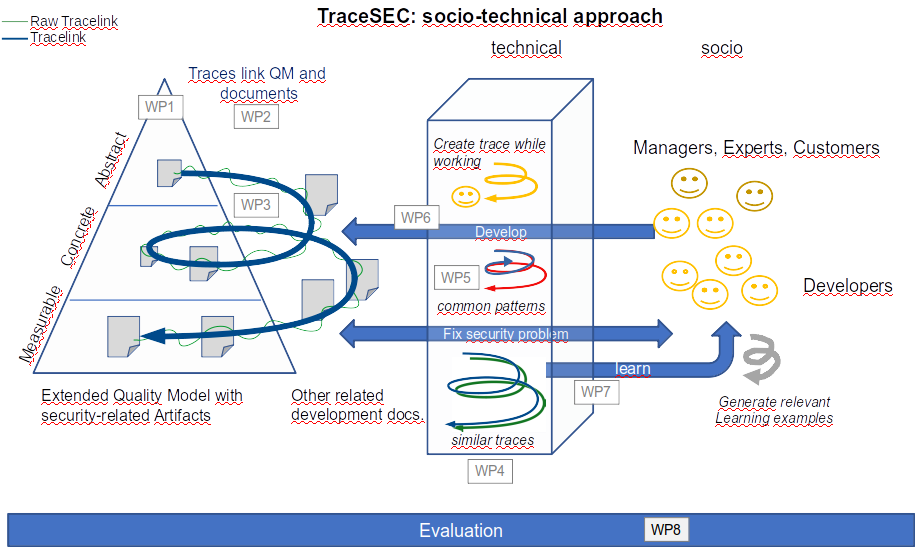
\includegraphics[width=1.0\textwidth]{resources/work-plan}
	\caption{Symolic representation of the TraceSEC-methods and its core components}
	\label{fig:work-plan}
\end{figure}

The work programme is organized around this structure. It starts from exploring and investigating what could and what should be added to an extended quality model for the three supported core activities (WP1). This will result in a reference model. It can be extended by trace links. Two issues are related: In WP2 we will identify and evaluate ways of collecting traces as a by-product. Whenever developers or stakeholders conduct a security-related activity, traces should be derived without extra effort. Given those raw traces, WP3 will develop and investigate techniques for assessing the relevance of trace elements. They will be classified, interpreted, and abstracted to reusable units of knowledge (centered around a scenario). WP 4 will explore high-level interpretations of threads of traces, that are meaningful to the stakeholders. In WP5-7, the above-mentioned three core activities in TraceSEC will be investigated with respect to the quality models, traces, and scenarios derived from them. WP5 is an ordinary development step which may or may not have security relevance. This can be decided by heuristic or automated classifiers, which may require additional human evaluation. WP6 represents the detailed diagnosis and analysis of a current security problem. Both WP5 and WP6 build on identification of patterns and similarities of scenarios (documents and threads). Information can be extracted from several similar threads. Workplace learning can be supported by offering highly contextualized examples and exercises; they will also be generated from the same web of traces and scenarios. Since they stem from that same context, they are implicitly highly relevant for this context. WP 7 will generate valuable educational material from threads for developers in their development context.

\begin{tabular}{|p{6cm}|p{10cm}|}
	\hline 
	\textbf{Work package} & \textbf{Deliverable} \\ 
	\hline 
	WP1: Security-Related Contents of a fine-grained QM & 1-Report/publication: What can be included, potential benefit, evaluation results.\\
	2-Reference model. \\ 
	\hline 
	WP2: Creation of Trace-Links as a By-Product of Activities & List of useful content items and how they can be captured as by-product (report) \\ 
	\hline 
	WP3: Interpretation of Trace-Links (relevance, abstraction, classification) & Report and associated demonstration software: Techniques and mechanisms for interpreting raw trace links (software demonstrators, process for semi-automated parts) \\ 
	\hline 
	WP4: In-Depth Analysis of Artifacts, facilitated by QM and trace links & Report and associated demonstration software: Techniques and mechanisms for analysis \\ 
	\hline 
	WP5: What led to this error? Trace-based forensics &  \\ 
	\hline 
	WP6: Suggestion of security mechanisms and processes &  \\ 
	\hline 
	WP7: Contextualized learning & Algorithms and demonstrators for extracting relevant parts from traces/threads, and for transforming them to learning units (e.g. videos) \\ 
	\hline 
	WP8: Evaluation on Realistic Use Cases & Report on developer support and experience \\ 
	\hline 
\end{tabular} 

\paragraph*{WP1: Security-Related Contents of a Fine-Grained Quality Model}
Using a quality model as fundamental artifact is a key decision in TraceSEC. The purpose of a quality model usually is to represent those non-functional requirements [7] that can be assigned to quality attributes that are important for a given project. Depending on the size of the project and on the significance of those quality aspects, the selection will be made by or together with customer representatives. There are formal and informal representations, automated and semi-automated techniques. In the case of market-driven development [13], the development organization has to decide, for example, on the relative importance of security vs. ease of use (see Running Example). 

As described above, not all projects detail quality models beyond this first layer of prioritization. In TraceSEC, we rely on a second layer of concrete components or use cases or situations and threats in which security is essential and where security requirements can be understood in more detail. This is the basis of a third layer of indicators and metrics (measurement) of those particular sub-aspects of security. On all layers, there may be other quality aspects, refinements, and metrics, too. If they are related or in contrast with security, we also want to represent this in our extended quality model. However, other quality aspects will only be represented where they relate to security, too. In contrast to most projects, our reference model for quality (including security) will be extended to include or reference (in separate artifacts) all heuristics, rationale, and mechanisms related to security. 

It is the purpose of WP1 to collect elements and aspects of security, reaching from requirements and priorities to vulnerable code patterns and heuristics for monitoring. There are two basic activities in WP1: (1) gathering candidates and (2) evaluating their relevance and significance. While (1) will be supported by our own experience from previous projects, an update of earlier literature reviews \todo[inline]{REFhabenWirEine?} and input from companies, (2) will identify irrelevant candidates and candidates that are doublets or will not advance research (exclusion criterion). The principal inclusion criterion for relevance will be whether we can find a use case or misuse case that references this kind of element. We do not seek completeness, but rather want to cover a broad range of definitely useful elements. This choice will lead to a rich selection of elements, but limit effort to a feasible level for a basic research project. 

This reference model with rationale and application examples will be the basic building material for projects. They will instantiate the elements, which will be a socio-technical activity: human decisions on informal levels will be included as much as technical monitoring and formal analysis.

Since all adopted elements in this rich quality model must be justified by their occurrence in a relevant product development, it will be possible to map them back to real projects. At this point, we do not distinguish by project characteristics or type, as long as the relevance is substantiated. 

The research questions in WP1 are:
\begin{description}
	\item[RQ1.1] What are relevant elements associated with security, and how can they be organized within extended quality models?
	\item[RQ1.2] How can information be organized in quality models to be usable for both humans and machines?
\end{description}

Deliverable:  
\begin{description}
\item[D1.1] Reference model and catalogue of elements.
\end{description}

The result of WP1 is a reference model with relevant elements identified, and a link or reference or example to the witnessing application in which it showed its relevance. Resulting instantiations (quality models) will be the source and reference for security knowledge in all three core activities. These knowledge elements will be connected by trace links (WP2, 3).


\paragraph*{WP2: Creation of Trace-Links as a By-Product of Development Activities}
In WP1, we collect and analyze security-related elements in a software project. Their relevance is supported by examples, but we do not investigate in WP1 how those elements are created or how they depend on each other in detail. WP2, in contrast, will identify sources and techniques to elicit security-related traces on all levels. This challenge will be addressed with a spectrum of socio-technical approaches. In the early or visionary phases of a project, there will be more informal considerations.

In traditional processes or agile processes, different kinds of artifacts are created and different kinds of tools are used. Different traces can be elicited, and they come in a different order. In this work package we investigate how these differences affect the elicitation as a by-product and how the traces can be made available for the following interpretation and analysis.

Example: They may lead, e.g., to top-layer decisions in the Running Example to prioritize security higher after the incident with the router. While the decision by itself may reside on the top layer of the quality model (“security is high priority. Rationale: Leaks may threaten personal medical data (GDPR)”), we will try to trace this decision from its triggers (the incident and a press release) over considered options (see Example) to the final resolution (“prioritize higher”) and its consequences.

Identification will include a variety of sources. The goal of WP2 is to include at least one instance of each type:
\begin{enumerate}
\item Explicit traditional traces from tools like Doors REF. They constitute the current state of practice in advanced projects. Less advanced projects often neglect traces at all.
\item  Automated repository mining: Patterns of reading-activity-writing indicate an information flow from the read to the written elements. 
\item  Negotiations among stakeholders about relative importance of quality aspects (e.g., usability vs. security) must be captured in a different way. We have experience in constructing tailor-made and privacy-respecting observation apps REF. They may, for example, require basic manual entries that are anonymized and pre-evaluated before they are ever stored.
\item  Interactions of developers during security-related development activities could be monitored technically or semi-automated, as sketched in (c).
\item  When developers interact with tools (e.g., CogniCrypt for generating secure code or nnnOtherTool), capturing a detailed trace automatically should be easier, but must be weighed with personal and privacy concerns.
\item  Run-time monitoring is yet another source of fine-grained traces. Again, not everything that can technically be collected should be included. It will be one of the questions in WP2 to investigate potentials and balance with effort and competing concerns.
\item  We will use established mining techniques REF and integrate informal traces from (a) and (c) using the information flow visualization technique FLOW [29] [31] to gain an overview and a socio-technical model of what is being elicited.
\end{enumerate}

It is important not only to elicit implausible or meaningless traces, but also to keep the number of traces as low as possible, to avoid the risk of bad maintenance or bad performance of any technical processing of traces.

Research Questions:
\begin{description}
\item[RQ2.1]  What are (existing or new) mechanisms for capturing traces that can be used to connect the security elements identified in WP1
\item[RQ2.2] How can raw traces be cleaned and filtered to achieve plausible and meaningful traces only?
\item[RQ2.3] How do different types of development processes affect the creation of trace links?
\end{description}

Deliverables: 
\begin{description}
\item[D2.1] A catalogue of elicitation techniques and related types of traces that are security-related and touch on elements of the extended quality models (WP1). 
\item[D2.2] Techniques (description and software demonstrators) for filtering out useless and implausible traces or parts of traces.
\end{description}

The result of WP2 is a catalogue of all identified elicitation techniques and techniques for filtering traces They can be used to build up a model of relevant “raw” traces, with connections to the QM, ready to be interpreted and analyzed in WP3 and 4.

\paragraph*{WP3: Interpretation of Trace Links for Adding Value}
In WP1, elements (models, decision, algorithms and heuristics) are identified. They are connected in the context of original use through traces extracted in WP2. Both WP1 and WP2 focus on finding opportunities and filtering out implausible and overly voluminous elements and traces. The resulting set can now be prepared for reuse and value-added exchange between the three core activities (development, problem analysis, learning). 

We will explore operations on traces that connect quality model elements and artifacts. We call these constructs “threads”. These operations are specific for the intended use in TraceSEC, but not limited to a single use within TraceSEC.

Examples include:
\begin{itemize}
\item Apply semantic filtering of traces. Longer sequences that do not touch on security elements can be hidden or removed. This helps to abstract to a higher level and reach a better overview. 
\item Soft matching of threads. If there are sub-sequences of common or similar security activities and elements in different traces, it may be interesting to look at the rest. For example, if a project starts with the same unusual repetition of decisions as a previous one, it could be interesting to see how that earlier project continued.
\end{itemize}

All operations can be used in at least one of the specific areas covered by WP6 (development), WP5 (problem analysis), and WP7 (learning). In most cases, they assist in preparing and reusing knowledge across these three core activities of TraceSEC. WP3 turns raw threads in meaningful ones.

Research Questions
\begin{description}
	\item[RQ3.1]	What are effective techniques to carry out operations on threads, as exemplified above?
	\item[RQ3.2]	How do machine learning techniques perform for this specific purpose, compared to socio-technical techniques that combine automated matching with human involvement?
\end{description}

Deliverable
\begin{description}
	\item[D3] Report on algorithms and mechanisms investigated, with study design and empirical results for comparison. 
\end{description}

The resulting report of WP3 covers both research questions, since RQ3.2 refines RQ3.1. 

\paragraph*{WP4: In-Depth Analysis of Artifacts, Facilitated by QM and Trace Links}
WP4 continues the semantic analysis. While WP1 and WP2 have removed implausible elements, WP3 entered the level of semantics, by investigating thread-specific operations that can be used for several purposes. WP4 goes beyond generic operations and explores options for analysis that is meaningful for project participants.

\textbf{Higher-level semantic interpretations of a thread} include:

\subparagraph*{Does a given thread from development comply to a given development process?} This question will use a simplified set of indicators for compliance. For example, Zazworka et al. [37] checked a development repository and analyzed whether there were always tests committed before source code. This was interpreted as a compliance criterion for test first. It is important to note that there is a trade-off between simple criteria and reliable results. In this example, Zazworka et al. did not check which tests referred to what part of code. Simplification was prioritized over reliability; in other words, only clear violations were to be reported (e.g., if there was no test at all before coding started).

\subparagraph*{Is this sequence of reading and writing artifacts or security elements typical?} In this type of question, there is no predefined process. The growing set of threads constitutes what is considered “typical”. We will apply machine learning for the statistical part of the analysis. Following our socio-technical approach, human interventions may be considered, too.

\subparagraph{Is a quality model populated in an unexpected way?} Patterns can be searched on threads (above) but also on elements of the quality model. For example, a quality model with lower-layer elements only (monitors, but no prioritization or concrete examples) may be too technology-focused, missing strategic awareness. This can in turn indicate a risk of ignoring other vulnerabilities, due to tunnel vision.

There are many hypotheses and experiences that can \textbf{evaluate a situation formalized on sets of threats}: Can we interpret repetition in a thread as problem fixing, or revision of a decision? This type of questions will probably lead to heuristics. 

Research Questions
\begin{description}
	\item[RQ4.1]	Is it feasible to recognize higher-level semantic similarities and potential problems by comparing and merging threads?
	\item[RQ4.2]	How can information captured in the quality models be utilized to provide more sophisticated low-level security checks?
\end{description}
	
Deliverable
\begin{description}
	\item[D4]	Scientific report (publication) on the Research Question. Feasibility would be demonstrated with at least two examples.
\end{description}

\paragraph*{WP5: What Led to This Error? Trace-based Forensics}
Security problems often have several causes that must come together. In the Running Example, nnn.
It is particularly difficult to reconstruct and diagnose the root causes of an attack or a privacy problem. An important precondition is a good record of potentially relevant events and decisions. Fine-grained tracing can be helpful. While it is difficult to remember details, and join them with details of another cause, threads may help – in particular since they are not limited to threads within a repository or on a computer. We envision socio-technical threads on all aspects of security.

Using the types of elements (WP1), traces (WP2), plausible (W3) and pre-interpreted threads (WP4) mentioned above, WP5 addresses one of the core activities related to security: Diagnosis and analysis of problems, which could be called trace-based forensics.

WP4 has two parts (leaving a trace and using a trace):
\begin{itemize}
\item Whenever forensic analysis of a real problem occurs, security experts search the (extended!) knowledge-base for symptoms and causes. This activity is human-driven and exploits the rare resource of security experts. Their experience enables them to identify suspicious parts faster. As they do that, they leave a trace. 
\item Earlier traces can be used to inspire less-experienced developers in problem analysis. Using soft matching from WP3 and WP4, they can reuse similar threads to look at the right places.
\item Following the model of FOCUS [21] [34], a new search can again create a trace. After the first steps, it is only a partial trace. Nevertheless, soft-matching the prefix against successful solution threads can help to identify promising threads to continue with. 
\item Perfect matches and a ready-made solution based on old cases will be the exception rather than the rule. However, much can be done on the side if most tracing and soft-matching does not require human effort (by-product [24]). That leaves human capacity for closing the gap between reused knowledge (threads) and actual problem context (thread again).
\item Entire sets of forensics can be collected. They represent typical cases and implicitly represent how frequently they occur in this environment. 
\end{itemize}

Research Question
\begin{description}
	\item[RQ5]	How effective are threads as knowledge representation for future problem analysis?
\end{description}
	
Deliverable
\begin{description}
	\item[D5] Report on effectiveness, potential, identified limits of thread-based problem analysis
\end{description}

\paragraph*{WP6: Suggestion of Security Mechanisms and Processes}
\begin{itemize}
\item Klare Empfehlung aus den alten QMen (anonymisiert), was sich bewährt hat
\item Code generieren
\item Heuristcs für Monitoring und Laufzeitfehler
\item Kriterien-Beispiele, um etwas zu beurteilen
\item Fälle aus anderen (anonymisierten) Artifacts, Testfällen usw., wie man weiterarbeiten kann.
\item Resultat:  Recommendations for current development
\end{itemize}

\paragraph*{WP7: Contextualized Learning}
There is a growing number of security lectures at Universities. Novice developers have a better likelihood to be aware of security. However, they are still a minority, and even that minority needs to keep learning, as attack knowledge grows and poses new security challenges. Learning on security is a continuous necessity, and it should consist of individual and organizational contributions to be effective.

WP7 will pick up general operations from WP3 and higher-level matching and interpretation from other work packages. Based on all these materials and thread-based knowledge representation, TraceSEC enables concrete and contextualized learning, closing the loop from development over problem analysis, to workplace learning on demand.

Learning on demand [6] occurs only when there is an actual demand, such as a security problem identified at run-time. Upon this trigger, the problem must be identified and solved. WP5 addresses this core activity. However, others can benefit from that solution.

WP7 has the vision to use appropriate threads (e.g., showing a problem and the process to solve it). They should be simplified (using mechanisms as developed in WP3 and WP4) and transferred to a representation that is better suited for learning. NnnREF presents guidelines for creating video tutorials. In [14], Karras and Schneider report on quality requirements and guidelines for creating “good-enough video” in software engineering. For WP7, it will be essential to strip threads of ballast and to re-construct a story. If there are multi-media elements in the quality model (WP1), they can be used; fine-grained technical traces from the repository may not include screen casts. But they can easily be generated or re-created following a detailed trace. FOCUS exemplifies a strategy to capture video as a by-product of demonstrating a prototype. 

WP7 will collect requirements for getting valuable educational material as by-product. We expect to implement some of those requirements in a socio-technical demonstrator, again combining the strengths of computers and humans. Additional information should be captured in a light-weight way, such as the cost and consequences of an error, external events.

As usual for organizational learning, individual learning is a crucial ingredient [26]. To lift it to an organizational level, some of the knowledge must be externalized [17] and stored in a repository for other members of the organization. In TraceSEC, the collection of threads constitutes the representation to store knowledge. More than simply storing it, the above-mentioned work packages investigate thread-based opportunities to benefit from core activities of others, and from sophisticated socio-technical support developed in TraceSEC.

Research Questions
\begin{description}
	\item[RQ7.1]	Do threads contain sufficient material to construct educational examples (maybe manually)?
	\item[RQ7.2]	How could existing parts be collected and transferred automatically, indicating what remains to be done by humans?
	\item[RQ7.3]	How can user decisions and changing public knowledge be automatically reflected in future automatically executed analyses.
\end{description}

Deliverables
\begin{description}
	\item[D7] Case study showing the feasibility of transfer. Maybe semi-automated. 
\end{description}

\paragraph*{WP8: Evaluation on Realistic Use Cases}
Our approach includes technical artifacts that can be continuously improved over time, and it also includes humans with different levels of experience who learn during the application of our approach. Therefore, an exactly repeatable case study is not achievable. To evaluate the overall approach regarding the project objectives, we will conduct user studies with realistic use cases, based on our experience with industry partners \todo[inline]{hier eine bessere Formulierung finden}.

The user studies will include developers with different levels of experience that use our approach and tool prototype in a set up development environment for a given set of tasks. Their activities and the recommendations and activities of the software will be logged as well as the intentions of the users using the thinking aloud technique \cite{thinkingAloud}. A control group will execute the same tasks without the approach. We expect the results of the treatment group to be better than the control group, because they have additional support. Interesting is the degree of developer support, measured in the number of successfully finished tasks and the time required, and the subjective experience of the developers in both groups using the thinking aloud protocol.

Research Questions
\begin{description}
	\item[RQ8.1]	Does the approach increase developer efficiency and effectiveness, and to which degree?
	\item[RQ8.2]	What are the experiences and thoughts of developers using the approach, compared to developers that do not use the approach?
\end{description}

Deliverables
\begin{description}
	\item[D8] Report on the evaluation
\end{description}

\paragraph*{Plan and Effort}
As outlined in Sec. nnn, the applicants approach the topic of TraceSEC from different angles: Jan Jürjens and his team has a long record of security modeling (e.g., in UMLsec [12]) and formal techniques to verify REF and ensure security REF. Kurt Schneider and his group focus on socio-technical aspects of software engineering, such as elicitation and validation of requirements and explainability [5]. They build tools to support the collaboration of technology and humans in a software engineering context (e.g., FOCUS [21], AppForMeetings, HeRA [11]). Their successful cooperation in SecVolution (SPP 1593) showed their ability to create solutions together that none of them could create on their own. 

As a consequence, work package leads are assigned to those focusing on a particular topic; however, both groups address their particular perspective in all work packages and will collaborate throughout all parts of the project. Therefore, the differences in planned person months is different between the groups, but not very different. The socio-technical approach requires constant exchange of ideas and results. Table nnn provides an overview of the effort devoted to the work packages by the two applicant groups. 

Table nnn:
\todo[inline]{Hier ein Vorschlag, in den WP 8 miteingerechnet ist und der etwas mehr Profil zeigt}

\todo[inline]{Hier die Tabelle mit den WP und PM}

Fig. nnn shows the distribution of effort in the planned work packages over time. Work progresses along work packages WP1-WP7. It is complemented by the cross-cutting evaluation work package WP8. Since both groups from Koblenz and Hannover work on different aspects of each work package, there is less need for parallel work packages. Of course, insights from a work package may lead to refine earlier work package results. This limited revision effort is planned in the latter work packages.

\todo[inline]{Hier ein Projektplan}

\subsection{Data handling}
%!TEX root = Beschreibung_des_Vorhabens.tex



\subsection{Other information\emptyheading}
% Hier ist Raum für weitere Angaben soweit sie nicht in den anderen Punkten aufgeführt werden konnten, aber aus Sicht der Antragstellerin bzw. des Antragstellers für diesen Antrag wichtig sind.
%[Text]%\input{2-5-weiteres}

\subsection{Descriptions of proposed investigations involving experiments on humans, human materials or animals as well as dual use research of concern}
%!TEX root = Beschreibung_des_Vorhabens.tex



\subsection{Information on scientific and financial involvement of international cooperation partners}
%!TEX root = Beschreibung_des_Vorhabens.tex

A substantial scientific and financial involvement of international project partners is not intended.

% -----------------------------------------------------------------------------------

\pagebreak

\section{Bibliography}
%\input{3-literatur}
\defbibheading{Lit}{\label{sec:literatur}}\vspace{-0.5cm}
\setlength\bibitemsep{0pt}
\begin{multicols}{2} 
	{\scriptsize
	\printbibliography[heading=Lit,notcategory=publikationen_juerjens, notcategory=publikationen_schneider,notcategory=publikationen-andere,notcategory=patente-angemeldet,notcategory=patente-akzeptiert]}
\end{multicols}
%

% -----------------------------------------------------------------------------------

\section{Requested modules/funds}
% Begründung jeder im Formular erfassten Position für jede Antragstellerin und jeden Antragsteller, unter Angabe von  Name, Vorname
%\input{4-mittel}

\subsection{Basic Module}

\subsubsection{Funding for Staff}


We request funding for \textbf{two doctoral researchers} (\emph{Doktorand*in}) for the full funding period. The doctoral researchers, supervised by the applicants and collaborating with other group members, will be mainly responsible for conducting the research as outlined in the work programme. 
One doctoral researcher will work at University of Koblenz-Landau covering ..., while the second doctoral researcher will be hosted at the Leibnitz University Hannover with a focus on .... Together with the applicants, the doctoral researchers will collaborate according to the work schedule outlined above.

Furthermore, we request funding for 
\textbf{student assistants} (\emph{wissenschaftliche Hilfskraft}, Bachelor's degree) with a total work load of xx h/week over the full funding period. They will help in ...
Since the tasks involve advanced software development, the assistants should have a Bachelor's degree in computer science or comparable. ... 

According to current DFG and local salary policies for 2019, we request the following funding:
\vspace{-4pt}
\begin{itemize} \setlength\itemsep{-0.4em}
	\item Two doctoral researchers (\emph{Doktorand*in}), full time, 36 month: \EUR{2 x 3 x 66\,300} = \textbf{\EUR{397\,800}}.
	% FB: different item for student assistants because usually different salaries

	\item Student assistants (\emph{wissenschaftliche Hilfskraft}, Bachelor's degree), xx h/week, 36 month at University of Koblenz-Landau (\EUR{x\,xxx}/month net costs): \EUR{xx x x\,xxx} = \textbf{\EUR{xx\,xxx}}
		\item Student assistants (\emph{wissenschaftliche Hilfskraft}, Bachelor's degree), xx h/week, 36 month at Leibnitz University Hannover (\EUR{xxx}/month net costs): \EUR{xx x xxx} = \textbf{\EUR{xx\,xxx}} 
\end{itemize}



\subsubsection{Direct Project Costs}
%\input{4-1-2-sachmittel}

\paragraph{Equipment up to €10,000, Software and Consumables\emptyheading}
%\input{4-1-2-1-geraete}

\paragraph{Travel Expenses}
%!TEX root = Beschreibung_des_Vorhabens.tex



\paragraph{Visiting Researchers}
% (ausgenommen Mercator-Fellow)
\input{4-1-2-3-gaeste}

\paragraph*{4.1.2.3--4.1.2.5\emptyheading}

%\paragraph{Mittel für Versuchstiere\emptyheading}
%%[Text]%\input{4-1-2-4-tiere}
%
%\paragraph{Sonstige Mittel}
%[Text]%\input{4-1-2-5-sonstige}
%
\setcounter{paragraph}{5}
\paragraph{Project-related publication expenses}
% 

\subsubsection{Instrumentation\emptyheading}

%\subsubsection{Investitionsmittel}
%[Text]%\input{4-1-3-investitionen}
%
%\paragraph{Geräte über 10.000 Euro}
%[Text]%\input{4-1-3-1-investitionen10}
%
%\paragraph{Großgeräte über 50.000 Euro}
%[Text]%\input{4-1-3-2-investitionen50}

\subsection*{4.2--4.7\emptyheading}

%\subsection{Modul Eigene Stelle}
%[Text]%\input{4-2-eigene}
%
%\subsection{Modul Vertretung}
%[Text]%\input{4-3-vertretung}
%
%\subsection{Modul Rotationsstellen}
%[Text]%\input{4-4-rotation}
%
%\subsection{Modul Mercator Fellow}
%[Text]%\input{4-5-mercator}
%
%\subsection{Modul Projektspezifische Workshops}
%[Text]%\input{4-6-workshop}
%
%\subsection{Modul Öffentlichkeitsarbeit}
%[Text]%\input{4-7-oeffentlichkeit}

% -----------------------------------------------------------------------------------

\section{Project requirements}
%  Für jede Antragstellerin und jeden Antragsteller, unter Angabe von Name, Vorname, Dienststellung (bei befristetem Arbeitsvertrag Angaben zur Laufzeit und ggf. zum Zuwendungsgeber)

\subsection{Employment status information}
%  Für jede Antragstellerin und jeden Antragsteller, unter Angabe von Name, Vorname, Dienststellung (bei befristetem Arbeitsvertrag Angaben zur Laufzeit und ggf. zum Zuwendungsgeber)
\textbf{Jan Jürjens} is a ...

\textbf{Kurt Schenider} is a ...

\subsection{First-time proposal data}
%\input{5-2-erstantrag}

\subsection{Composition of the project group}
% Angabe nur der Personen, die im Projekt mitarbeiten, aber nicht aus diesem finanziert werden, mit Name, akademischem Grad, Dienststellung und Art der Finanzierung
\vspace{-5pt}
\noindent\begin{tabularx}{\textwidth}{lX}
	{\bf Koblenz-Landau}  & \vspace{-0.68cm}\begin{itemize} \setlength\itemsep{-0.4em}
		\item \textbf{Prof. Dr. Jan Jürjens} (applicant/principle investigator), full professor, group leader
		\item \textbf{N.N.}, doctoral researcher, funded by the proposed project\vspace{-0.6cm}
	\end{itemize} \\
	\\
	{\bf Hannover} & \vspace{-0.68cm}\begin{itemize} \setlength\itemsep{-0.4em}
		\item \textbf{Prof. Dr. Kurt Schneider} (applicant/principle investigator), full professor, group leader
		\item \textbf{N.N.}, doctoral researcher, funded by the proposed project\vspace{-0.6cm}
	\end{itemize}
\end{tabularx}

\subsection{Cooperation with other researchers}

\subsubsection{Researchers with whom you have agreed to cooperate on this project}
Within the proposed project, we plan to collaborate closely with the following researchers. They contribute additional experience in different areas to the project. 
\vspace{-5pt}
\begin{itemize}\setlength\itemsep{-0.4em}
	\item \textbf{? ? }, University of ?-- supporting with expertise in \ldots.
\end{itemize}
%\input{5-4-1-zusammenarbeit}

\subsubsection{Researchers with whom you have collaborated scientifically within the past three years}
%!TEX root = Beschreibung_des_Vorhabens.tex

\textbf{Jan Jürjens} has collaborated with ...

\textbf{Kurt Schneider} has collaborated with ...


%\subsection{Scientific equipment}
% Angaben zu den für das Projekt zur Verfügung stehenden größeren Geräten (ggf. auch Großrechenanlagen, wenn Rechenleistung benötigt wird)
%\input{5-5-apparate}

\subsection*{5.5--5.7\emptyheading}

%\subsection{Projektrelevante Beteiligungen an erwerbswirtschaftlichen Unternehmen\emptyheading}
%% Angaben zum Zusammenhang des Projekts mit dem Produktbereich des Unternehmens
%% [Text]%\input{5-6-unternehmen}

% -----------------------------------------------------------------------------------

\section{Additional information}
% Bitte informieren Sie die DFG hier insbesondere - sofern zutreffend - über bereits an anderer Stelle eingereichte Anträge bzw. Anträge mit Großgeräten.
We did not request any funding for this research project or parts of it at a third party.

\end{document}
